% !TEX root = ../agglo_clust_review.tex

\section{Generalized framework for agglomerative clustering of signed graphs} \label{sec:general_framework}
% In this section, we first define notation and then introduce one of our main contributions: a signed graph partitioning algorithm (Sec. \ref{sec:algorithm}) that can be seen as a generalization of several existing and new clustering algorithms (Sec. \ref{sec:alg_update_rules}).

\subsection{Notation} \label{sec:notation}

\textbf{Graph formalism} -- We consider an undirected simple edge-weighted graph $\mathcal{G}(V,E,w^+, w^-)$ with both attractive and repulsive edge attributes.
% In computer vision applications, the nodes can represent either pixels, superpixels or voxels.  
The weight function $w^+: E \rightarrow \mathbb{R}^+$ associates to every edge a positive scalar attribute $w_e^+\in \mathbb{R}^+$ representing a merge affinity or a similarity measure.
% the higher this number, the higher the inclination of the two incident vertices to be assigned to the same cluster\footnote{Note that other formalisms for positively weighted graphs associate distances to the edges, thus, the \emph{lower} the edge weight, the higher the attraction between the two linked nodes, contrary to our definition of $w^+$.}. 
On the other hand, $w^-: E \rightarrow \mathbb{R}^+$ associates to each edge a split tendency $w_e^- \in \mathbb{R}^+$.
% : \OPTIONAL{the higher this number, the higher the inclination of the two incident vertices to be assigned to different clusters}.
% the higher this weight, the more the incident vertices would like to be in different clusters. 
Graphs of the type $\mathcal{G}(V,E,w^+, w^-)$ are often defined as \emph{signed graphs} $\mathcal{G}(V,E,\cost)$, featuring positive and negative edge weights $\cost_e\in \mathbb{R}$. Following the theoretical considerations in \cite{lange2018partial}, we define signed weights as ${\cost_e = w_e^+ - w_e^-}$. 
% Some approaches directly compute $\cost_e$, whereas others compute $w_e^+$ and $w_e^-$ separately.
% In this formalism, graphs with purely attractive interactions are a special case of $\mathcal{G}(V,E,\cost)$ with $\cost_e \geq 0, \, \forall e \in E$. 

\textbf{Multicut objective} -- We call the set $\Pi$ a \emph{clustering} or \emph{partitioning} with $K$ clusters if $V = \cup_{S\in\Pi} S $, $\,S \cap S' = \emptyset$ for different clusters $S, S'\in \Pi$ and every cluster $S \in \Pi$ induces a connected subgraph of $\mathcal{G}$. 
For any clustering $\Pi$ of $\mathcal{G}$, we denote as $E^0_\Pi= \{ e_{uv} \in E \,|\, \exists S \in \Pi : u,v \in S \}$ the set of edges linking nodes in the same cluster, and as $E_\Pi^1= E \setminus E^0_\Pi$ the set of edges whose linked nodes belong to distinct clusters, which is known as the \emph{multicut} of $\mathcal{G}$ associated to clustering $\Pi$. The instance of the NP-hard \emph{minimum cost multicut problem} w.r.t. $\mathcal{G}(V,E,w_e)$ is the task of finding a clustering that optimally balance the attraction and repulsion in the graph and is given by the following binary integer program:
% \begin{equation}
% E_\Pi^0 \equiv \{ e_{uv} \in E \,|\, \exists S \in \Pi : u \in S \, \text{and} \, v \in S \}, \qquad E^1_\Pi \equiv E \setminus E^0_\Pi.
% \end{equation}
% \begin{align}
% E_\Pi^0 &= \{ e_{uv} \in E \,|\, \exists S \in \Pi : u \in S \, \text{and} \, v \in S \}, \\
% E^1_\Pi &= E \setminus E^0_\Pi.
% \end{align}
\begin{equation}\label{eq:MC_objective}
% \min_\Pi \texttt{MC}(\Pi) \equiv
 \min_\Pi \sum_{e\in E} \cost_e x_e^\Pi,  \qquad \text{where} \quad x^\Pi_e = 
 \begin{cases} 
 1 & \text{if } e\in E^1_\Pi \\
 0 & \text{otherwise}.
 \end{cases}
\end{equation}
% In the next chapters we will use this objective as a way to measure how balanced is a clustering found by the tested agglomerative clustering algorithms.


\textbf{Linkage criteria and hierarchical trees} -- 
% We also denote as $S_u$ the cluster associated with node $u$ \TODO{Needed?}.
% We call two clusters $S,S'$ \emph{adjacent} if there exists at least one edge ${e_{ts}\in E}$ connecting a node $t\in S_u$ to a node $s\in S_v$. 
Let the interaction $\interact(S,S')$ between two clusters $S,S'$ be defined as a function $\interact{}:2^{V} \times 2^{V} \rightarrow \mathbb{R}$, named \emph{linkage criterion}, depending on the weights of \emph{all} edges connecting clusters $S$ and $S'$, i.e. ${(S \times S') \cap E}$. 
The linkage criteria tested in this article are listed and defined in Table \ref{tab:linkage-criteria}.
A \emph{dendrogram} $T$ is a rooted binary tree\footnote{In general, one could look at trees that are not binary. However, the algorithms discussed in this paper always generate binary hierarchical trees, so nothing would be gained by this generalization.} representing the merging order of an agglomerative algorithm, such that the leaves of the tree are in one-to-one correspondence with $V$. 
Let $T_{\mathrm{R}},T_{\mathrm{L}}\subset T$ denote the subtrees rooted at the two children of the root node in $T$.
For any two leaves $u,v \in V$, let $T[u \vee v]$ be the subtree rooted at the least common ancestor $(u \vee v)\in T$ of nodes $u$ and $v$ (furthest from the root), and let \texttt{leaves}$(T[u \vee v])\subseteq V$ be the set of leaves of this subtree. 
% \TODO{Here we talk about the algorithm already, so we could move it to next section and the flow could be better. But we need a tree in the alg. So we better do this later}
% Algorithm \ref{main_alg} returns a binary tree denoted by $T^*$.
Given an agglomerative algorithm with merging tree $T$, let $h_T:T \rightarrow \mathbb{N}$ denote the \emph{dendrogram-height} of each $(u\vee v)\in T$, which is defined as the iteration number at which nodes $u,v\in V$ were merged by the algorithm (\TODO{Fig.~1}). We also define $\treeHeight(u,v)$ as the signed interaction $\interact{}(S,S')$ between the two clusters $S,S'$ that were merged at iteration $h_T(u\vee v)$: 
% Then, given a binary tree $T$ and a linkage criterion $\interact$, we can associate a \emph{signed similarity} function $\treeHeight$ to each pair of distinct original nodes $u\neq v$, with $u, v \in V$:
\begin{equation}\label{eq:def_dendr_interact}
\treeHeight(u,v) \equiv \interact{} \big( \text{\texttt{leaves}}(T_{\mathrm{R}}[u \vee v]), \text{\texttt{leaves}}(T_{\mathrm{L}}[u \vee v]) \big)
\end{equation}
% \OPTIONAL{In other words, $h_T(u,v)$ and $\treeHeight(u,v)$ represent the \emph{dendrogram-height} and \emph{signed-interaction} associated to each $u \vee v$ node in the tree $T$ (see toy example in \TODO{Fig.~1}).}




% \begin{algorithm}[t]
%   \caption{\algname{}: generalized algorithm for signed graph partitioning}
%    \hspace*{\algorithmicindent} \textbf{Input:} Graph $\mathcal{G}(V,E,w^+,w^-)$; linkage criterion $\interact{}$; boolean {\color{blue}\texttt{addCannotLinkConstraints}}  \\
%   \hspace*{\algorithmicindent} \textbf{Output:} Final clustering $\Pi$\\
%   \hspace*{\algorithmicindent} 
%   \begin{algorithmic}[1]
%       \State Initialize clustering $\Pi=\{\{v_1\}, \ldots, \{v_{|V|}\}\}$ with each node in its own cluster
%       \State Initial interactions between nodes given by $\cost_e = w^+_e - w^-_e$
%       \Repeat
%         \State Select pair of clusters $S_u,S_v\in\Pi$ with highest absolute interaction $|\interact{}(S_u,S_v)|$
%         \If{\big[{\color{ForestGreen}\textbf{$\interact{}(S_u,S_v) > 0$}}\big] \textbf{and} \big[$S_u,S_v$ are \textbf{not} constrained\big]}
%           \State Merge cluster $S_u$ with $S_v$: update interactions and cannot-link constraints with all their neighbors
%         \ElsIf{\big[{\color{red}\textbf{$\interact{}(S_u,S_v) \leq 0$}}\big] \textbf{and} {\color{blue}\texttt{addCannotLinkConstraints}}}
%           \State Add CannotLink Constraint between clusters $S_u$ and $S_v$
%         \EndIf
%       \Until{\big[all interactions between clusters are repulsive\big] \textbf{or} \big[all adjacent clusters have cannot-link constraints\big]}
%       \State
%       \Return $\Pi$
%   \end{algorithmic}
%   \label{main_alg}
% \end{algorithm}



\subsection{The \algname{} algorithm} \label{sec:algorithm} 
% : generalized agglomerative algorithm for signed graph partitioning

Our main contribution is a generalized agglomerative algorithm for signed graph partitioning (GASP) that generalizes hierarchical clustering (HC) to signed graphs. 
The framework, defined in the following, encompasses several known and new agglomerative algorithms on display in Table \ref{tab:linkage-criteria}, which are differentiated by the linkage criterion employed, similarly to HC.

In Algorithm \ref{main_alg}, we provide simplified pseudo-code for the proposed \algname{} algorithm. \algname{} implements a bottom-up approach that starts by assigning each node to its own cluster and then iteratively merges pairs of adjacent clusters. The algorithm proceeds in three phases. 

In \emph{Phase~One}, \algname{} selects the pair of clusters with the highest absolute interaction $|\interact(S, S')|$, so that the most attractive and the most repulsive pairs are analyzed first. If the interaction is repulsive and the algorithm option \emph{addCannotLinkConstraints} is \texttt{True}, then the two clusters are constrained so that their members can never merge in subsequent steps of \emph{Phase~One}. If the interaction is attractive, then the clusters are merged, provided that they were not previously constrained. 
After each merge, the interaction between the merged cluster and its neighbors is updated according to one of the linkage criteria $\interact(S, S')$ listed in Table \ref{tab:linkage-criteria}. \emph{Phase~One} terminates when all the remaining clusters are either constrained or share repulsive interactions.

\emph{Phase Two:} Now that the clusters have grown in size, the algorithm removes the constraints previously introduced in \emph{Phase~One} and merges all the clusters that still share an attractive interaction, merging the most attractive one first\footnote{Note that in the version of \algname{} with \emph{addCannotLinkConstraints} set to \texttt{False}, nothing happens in \emph{Phase~Two}.}. The final clustering $\Pi^*$ returned by \algname{} is found at the end of \emph{Phase~Two} and it is then composed of clusters sharing only mutual repulsive interactions. 

Finally, in \emph{Phase~3}, the algorithm keeps merging all clusters until only a single one is left and then returns the hierarchical tree $T^*$ representing the full sequence of merging steps.
The algorithm was implemented using a standard HC implementation with computational complexity $\mathcal{O}(N^2 \log N)$ (see Appendix \ref{sec:detailed_impl} for more details). 


% , we comment on the algorithm's computational complexity $\mathcal{O}(N^2 \log N)$ and present our implementation given by the edge contraction Algorithm \ref{detailed_alg} based on a \emph{disjoint set data structure} and a \emph{priority queue}.

\begin{algorithm}[t]
\footnotesize
  \begin{flushleft}
  \footnotesize
  \caption{\algname{}}
  % \caption{\algname{}: generalized algorithm for signed graph partitioning}
   \hspace*{\algorithmicindent} \textbf{Input:} Graph $\mathcal{G}(V,E,w^+,w^-)$; linkage criterion $\interact{}$; \\ 
   \hspace*{4.3em}boolean {\color{blue}addCannotLinkConstraints}  \\
  \hspace*{\algorithmicindent} \textbf{Output:} Final clustering $\Pi^*$, rooted binary hierarchical tree $T^*$\\
  \hspace*{\algorithmicindent} 
  \begin{algorithmic}[1]
  \footnotesize
  % \small
      \State Initial clustering: $\Pi=\{\{v_1\}, \ldots, \{v_{|V|}\}\}$
      \State Initialize hierarchical tree $T$ with leaves nodes $V=\{v_1,\ldots,v_{|V|}\}$
      \State Initialize interactions between clusters with $\cost_e = w^+_e - w^-_e$
      \State \emph{// Phase 1: Merge positive interactions (possibly using constraints)}
      \State Push absolute interactions $|w_e|$ to priority queue $PQ$
      \Repeat 
        \State Pop $S,S'\in\Pi$ from $PQ$ with highest interaction $|\interact{}(S,S')|$
        \If{\big[{\color{green}\textbf{$\interact{}(S,S') > 0$}}\big] \textbf{and} \big[$S,S'$ \textbf{not} constrained\big]}
          \State Merge clusters $S$, $S'$ and update hierarchical tree $T$
          \State Update interactions \& constraints with neighboring clusters
        \ElsIf{{\color{blue}addCannotLinkConstr} \textbf{and}  \big[{\color{red}\textbf{$\interact{}(S,S') \leq 0$}}\big]}
          \State Add CannotLink Constraint between $S$ and $S'$
        \EndIf
      \Until{\big[$PQ$ is empty\big]}
      % \State
      % \If{{\color{blue}addCannotLinkConstr}} % \Comment{Step 2: release constraints}
      \State \emph{// Phase 2: Remove constraints \& merge all positive interactions}
      \State Push signed interactions $\interact{}(S,S')$ to PQ, $\forall S, S' \in \Pi$
      \Repeat 
        \State Pop $S,S'\in\Pi$ from $PQ$ with highest interaction $\interact{}(S,S')$
        \If{\big[{\color{green}\textbf{$\interact{}(S,S') > 0$}}\big]}
          \State Merge clusters $S$, $S'$ and update hierarchical tree $T$
          \State Update interactions with neighboring clusters
        \EndIf
      \Until{\big[{\color{red}\textbf{$\interact{}(S,S') \leq 0$}}\big]} 
      \State Save the final clustering $\Pi^* \gets \Pi$ 
      \State \emph{// Phase 3: Merge negative interactions until one single cluster is left}
      \Repeat
        \State Pop $S,S'\in\Pi$ from $PQ$ with highest interaction $\interact{}(S,S')$
        \State Merge clusters $S$, $S'$ and update hierarchical tree $T$
        \State Update interactions with neighboring clusters
      \Until{\big[Only one cluster is left in $\Pi$\big]} 
      % \EndIf
      \State
      \Return $\Pi^*$, $T^*\gets T$
  \end{algorithmic}
    \label{main_alg}
  \end{flushleft}

\end{algorithm}


\subsection{\algname{}: New and existing algorithms} \label{sec:alg_update_rules}


% \begin{prop} 
% The Mutex Watershed Algorithm (MWS) introduced by \cite{wolf2018mutex} and with empirical $\mathcal{O}(N \log N)$ complexity outputs the same clustering $\Pi^*$ returned by  the \algname{} Algorithm \ref{main_alg} with the use of cannot-link constraints and an Absolute Maximum update rule:
% \begin{equation}\label{eq:def_abs_max}
% f_{\mathrm{Abs.Max.}}(\tilde{\cost}_1,\tilde{\cost}_2) = \begin{cases} 
%             \tilde{\cost}_1 & \text{if}\,\, |\tilde{\cost}_1|>|\tilde{\cost}_2|\\
%             \tilde{\cost}_2 & \text{otherwise}
%              \end{cases} 
% \end{equation}
% \end{prop}
In this paper we focus on five linkage methods (see columns of Table~\ref{tab:linkage-criteria}). Many more linkage criteria have been applied to unsigned graphs \cite{nunez2013machine,felzenszwalb2004efficient,funke2018large}, involving median-based or size-regularized methods, but we decided to focus this paper on those five criteria because they represent the most known choices.  

\paragraph{Sum Linkage} -- 
An agglomerative algorithm with sum linkage does only make sense for graphs with signed edge weights, because only for these graphs the sum of two attractive (or repulsive) interactions is still attractive (repulsive). On positive weighted graphs, on the other hand, a strong attractive interaction could be obtained by summing many weak interactions, which is not desirable. Such an algorithm was pioneered in \cite{levinkov2017comparative,keuper2015efficient} and was named Greedy Agglomerative Edge Contraction (GAEC)\footnote{An algorithm equivalent to GAEC was recently independently re-proposed in \cite{chehreghani2020hierarchical}.}. All variations of \algname{} decrease the multicut objective defined in Eq.~\ref{eq:MC_objective} each time two clusters with positive interaction are merged. But only GAEC always makes the \emph{greedy-choice} that will mostly decrease the multicut objective at every step. The authors of \cite{levinkov2017comparative} also proposed a version of GAEC with cannot-link constraints named \emph{GreedyFixation}, but the constrained sum-link version of \algname{} proposed here (named \emph{HCC-Sum} in Table~\ref{tab:linkage-criteria}) did perform better in our experiments.

\paragraph{AbsMax Linkage} -- This linkage method is also specific to signed graphs, since on positive-weighted graphs it would be equivalent to single linkage. Here, we prove that the Mutex Watershed Algorithm \cite{wolf2018mutex} can be seen as an agglomerative algorithm with AbsMax linkage (see proof in Appendix):
\begin{prop} 
The \algname{} Algorithm \ref{main_alg} with AbsMax linkage (see def. in Table \ref{tab:linkage-criteria}) returns the same final clustering $\Pi^*_{\mathrm{AbsMax}}$ whether or not cannot-link constraints are introduced. In particular, $\Pi^*_{\mathrm{AbsMax}}$ is equal to the clustering returned by the Mutex Watershed Algorithm (MWS) \cite{wolf2018mutex}, which has empirical complexity $\mathcal{O}(N \log N)$. 
\end{prop}


\paragraph{Average, Single, and Complete Linkage} -- These three linkage criteria have been throughly studied on positive-weighted graphs. In \cite{chehreghani2020hierarchical}, the authors proved that applying these three linkage methods to a signed graph is equivalent to applying them to the positive-weighted graph obtained by shifting all edge weights by a constant.  Here, we prove which of the algorithms included in our generalized framework have this invariance-property: (proof in Appendix)
\begin{prop} \label{prop:weight_shift_invariant}
We call an agglomerative algorithm ``weight-shift invariant'' if the structure of the merging tree $T$ returned by such algorithm is invariant w.r.t. a shift of all edge weights $w_e$  by a constant $\alpha\in \mathbb{R}$. Among the versions of \algname{} studied in this paper, only those using Average, Single, and Complete linkage criteria without cannotLinkConstraints are weight-shift-invariant (see algorithms typeset in bold font in Table~\ref{tab:linkage-criteria}).
\end{prop}
\noindent To our knowledge, Avg, Single, and Complete linkage methods have never been combined with cannot-link constraints on signed graphs, so the algorithms that in Table~\ref{tab:linkage-criteria} are named \emph{HCC-Avg}, \emph{HCC-Single}, and \emph{HCC-Complete} are new.


% \textbf{Weight-shift hierarchical algorithms} -- Given an algorithm that outputs a clustering $\Pi$ for a signed graph $\mathcal{G}(V,E,w_e)$, we call the algorithm \emph{weight-shift hierarchical} if, by adding a constant $\alpha \in \mathbb{R}$ to all edge weights $w_e$, the algorithm outputs a clustering $\Pi'$ which is a coarsening of $\Pi$ when $\alpha>0$ and a refinement of $\Pi$ when $\alpha<0$\footnote{A clustering $\Pi'$ is a coarsening of $\Pi$ when every $S' \in \Pi'$ is the union of one or more clusters in $\Pi$. Similarly, $\Pi'$ is a refinement of $\Pi$ when every $S \in \Pi$ is given by the union of one or more clusters in $\Pi'$}.








% \ref{tab:linkage-criteria}, additional ones were proposed in the literature:
% \cite{nunez2013machine} for example uses a learned approach where a random forest classifier updates the cluster interactions depending on predefined edge and node features; other approaches introduce a weight regularization depending on the size of the clusters \cite{felzenszwalb2004efficient,kardoostsolving}, whereas 
% \cite{funke2018large} uses a \emph{quantile} linkage criterion by populating a histogram for each inter-cluster interaction. In our experiments, we decided to focus on the linkage criteria listed in Table \ref{tab:linkage-criteria}, since they represent the most common options.





% In the special case of an unsigned graph with only positive interactions, i.e. $w_e^-=0$ and $\cost_e \geq 0$ $\forall e\in E$, 
%  the algorithm performs a standard agglomerative hierarchical clustering by returning only a single cluster and a hierarchy of clusters defined by the order in which the clusters are merged (see Table \ref{tab:linkage-criteria}, unsigned graphs).

% Given a graph with both attractive and repulsive cues, an edge contraction algorithm with a sum update rule was pioneered in \cite{levinkov2017comparative,keuper2015efficient} (Table \ref{tab:linkage-criteria}, \emph{Sum} linkage). The authors present both a version with cannot-link constraints and one without, and then compare them with other greedy local-search algorithms approximating the multicut optimization problem.
% The Mutex Watershed \cite{wolf2018mutex} is another signed graph partitioning algorithm that introduces dynamical cannot-link constraints. In Proposition \ref{prop:equiv_MWS} (see Appendix \ref{sec:appendix_abs_max}) we prove that, surprisingly, it can also be seen as an efficient implementation of \algname{} with \emph{Absolute maximum} linkage (def. in Table \ref{tab:linkage-criteria}). Moreover, in Proposition \ref{prop:abs_max_cannot_link_property} we also prove that \algname{} with \emph{Abs Max} linkage returns the same clustering with or without enforcing cannot-link constraints.
% On the other hand, to our knowledge, \emph{Average}, \emph{Max} or \emph{Min} linkage criteria have never been used for signed graph agglomerative algorithms or been combined with cannot-link constraints.


\paragraph{Algorithms defining an ultrametric} -- The connection between agglomerative algorithms and ultrametrics\footnote{A metric space $(X,d)$ is an \emph{ultrametric} if for every $x,y,z \in X$, $d(x,y)\leq \max \{d(x,z), d(y,z)\}$.} is well known \cite{johnson1967hierarchical,milligan1979ultrametric}. Normally, ultrametrics are associated to strictly positive \emph{similarity} or \emph{dissimilarity} measures on a graph. Here, we generalize this concept to signed graphs. To do so, we first map the signed interaction $\treeHeight{}$ defined in Eq.~\ref{eq:def_dendr_interact} to positive ``distances'' $d_{T}:V \times V \rightarrow \mathbb{R}^{+}$:
\begin{align}\label{eq:UM_def}
d_{T}(u,v)\equiv &\begin{cases}
0 & \text{if}\,\, u=v\\
M-\treeHeight(u,v) & \text{if}\,\, u\neq v
\end{cases}\quad \forall u,v\in V\\
\mathrm{where}& \quad  M \equiv  \epsilon + \max_{u',v'\in V,\,u'\neq v'}\treeHeight(u',v')
\end{align}
and where $\epsilon > 0$. By definition, we have that $d_{T}(u,v)=d_{T}(v,u)$ and $d_{T}(u,u)= 0$. We then prove the following two propositions (proofs are left in Appendix):
\begin{prop}
Consider a graph $\mathcal{G}(V,E,w_e)$, a linkage criteria $\interact{}$, and an AC algorithm returning a binary rooted tree $T$ with height $h_T$. The quantity $(V, d_{T})$ defined in Eq.~\ref{eq:UM_def} is an ultrametric iff, $\forall u,v,t \in V$:
\begin{equation}
\interact{}_{T}(u,v) > \interact{}_{T}(u,t) \Leftrightarrow h_T(u \vee v) < h_T[u \vee t] 
\end{equation}
In words, $(V, d_{T})$ is an ultrametric iff the interaction $\interact{}_{T}(u, v)$ associated to the least common ancestor ${(u\vee v)\in T}$ is both lower than any other $(u\vee v)$-descendant node and higher than any other $(u\vee v)$-ancestor node in the tree $T$.
\end{prop}
\begin{prop}
% Consider the binary rooted tree $T^*$ returned by the \TODO{all variants in Table 1} \algname{} Algorithm~\ref{main_alg}, given a choice of linkage criteria $\interact{}$ and the use (or not) of CannotLinkConstraints. 
Among the algorithms listed in Table \ref{tab:linkage-criteria} and included in the \algname{} framework, only Mutex Watershed and hierarchical clustering with Average (HC-Avg), Single (HC-Single) and Complete linkage (HC-Complete) define an ultrametric given by the quantity $(V, d_{T^*})$ defined in Eq.~\ref{eq:UM_def}, where $T^*$ is the tree returned by Algorithm~\ref{main_alg}.
\end{prop}





% Apart from the linkage criteria defined in Table \ref{tab:linkage-criteria}, additional ones were proposed in the literature:
% \cite{nunez2013machine} for example uses a learned approach where a random forest classifier updates the cluster interactions depending on predefined edge and node features; other approaches introduce a weight regularization depending on the size of the clusters \cite{felzenszwalb2004efficient,kardoostsolving}, whereas 
% \cite{funke2018large} uses a \emph{quantile} linkage criterion by populating a histogram for each inter-cluster interaction. In our experiments, we decided to focus on the linkage criteria listed in Table \ref{tab:linkage-criteria}, since they represent the most common options.

% \begin{figure}[t]
% \centering
%         \begin{subfigure}[t]{0.46 \textwidth}
%         \centering
%         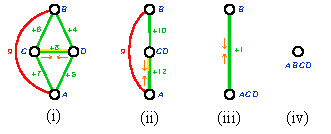
\includegraphics[width=\textwidth]{figs/example_no_constr.pdf}
%         \caption{No constraints}\label{subfig:no_constraints}
%     \end{subfigure} \hfill \vspace{8pt}
%     \begin{subfigure}[t]{0.46 \textwidth}
%         \centering
%         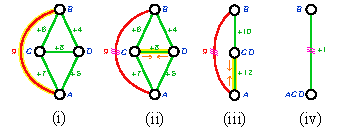
\includegraphics[width=\textwidth]{figs/example_with_constr.pdf}
%         \caption{With cannot-link constraints}\label{subfig:with_constraints}
%     \end{subfigure}
% \caption{Some iterations of the generalized algorithm (using \emph{Sum} linkage criteria) with and without adding cannot-link constraints. The graph has both attractive (green) and repulsive (red) edges and cannot-link constraints are shown with triple violet bars on the edges. The edge selected at each iteration is highlighted in yellow. We note that when constraints are enforced, the final clustering is given by two clusters instead of only one.}
% \label{fig:algorithm_with_without_CLC}
% \end{figure}


% \begin{table*}[t]
%     % \centering
%     \scriptsize
%     \begin{subtable}[t!]{\textwidth}\centering
%         \begin{tabular}{R{5em}  l | M{10em} | M{8em}  M{8em}}
%             \multicolumn{2}{c|}{\multirow{2}{*}[-0.5em]{\thead{\textbf{\algname{} linkage criteria}\\ $\,\,\interact(S_u ,S_v)$}}}  & \multirow{2}{*}[-0.5em]{\thead{\textbf{Unsigned} \\\textbf{Graphs}}} & \multicolumn{2}{c}{\thead{\textbf{Signed Graphs}}}  \\        
%             \multicolumn{2}{c|}{} &  &  \multicolumn{1}{c}{\thead{No \\Constraints}} & \thead{With\\ Constraints} \\        
      
%             \midrule
%              Sum: & $\displaystyle \sum_{e\in E_{uv}} \cost_e$ & \thead{Sum Linkage\\Hier. Aggl. Clust.} & \thead{GAEC \cite{keuper2015efficient}} & \thead{Greedy\\Fixation \cite{levinkov2017comparative}} \\ 
            
%              \makecell[r]{Abs. Max:} & 
%             $\displaystyle \cost_e$ with $\displaystyle e = \argmax_{t\in E_{uv}} |\cost_t|$
%                & \thead{Single Linkage\\Hier. Aggl. Clust.} & \thead{Mutex\\Watershed \cite{wolf2018mutex}} & \thead{Mutex\\Watershed \cite{wolf2018mutex}} \\
%              \makecell[r]{Average:} & $\displaystyle \sum_{e\in E_{uv}} \cost_e \bigg/ \big|E_{uv}\big|  $ & \thead{ Average Linkage\\ Hier. Aggl. Clust.} & \thead{\textbf{NEW}} & \thead{\textbf{NEW}}\\ 

%             Max: & $\displaystyle \max_{e\in E_{uv}} \cost_e$ & \thead{Single Linkage\\Hier. Aggl. Clust.} & \thead{\textbf{NEW}} & \thead{\textbf{NEW}}\\ 

%             Min:& $\displaystyle \min_{e\in E_{uv}} \cost_e$ & \thead{Complete Linkage\\ Hier. Aggl. Clust.}  & \thead{\textbf{NEW}} & \thead{\textbf{NEW}}
%         \end{tabular}
%     \end{subtable} 
%     \vspace{1em}
%     \caption{Existing and new clustering algorithms that can be reformulated as special cases of the proposed generalized algorithm for signed graph partitioning, \algname{}, given a linkage criterion, a type of graph (signed or unsigned) and the optional use of cannot-link constraints. The set $E_{uv}$ is defined as the set of all edges connecting cluster $S_u$ to cluster $S_v$, i.e. $E_{uv}=(S_u \times S_{v \neq u}) \cap E$.}
%     \label{tab:linkage-criteria}
% \end{table*}







% \begin{table}[t]
%     \centering
%     % \scriptsize
%     \tiny
%     \begin{subtable}[t!]{0.5\textwidth}\centering
%         \begin{tabular}{l  c  c  c  c  c}
%         \toprule
%         Dataset & HC-Avg & GAEC & MWS & Constr-Avg & Constr-Sum \\ \midrule
%         \emph{Image Seg.} \\
%         \emph{Knott-3D-150} \\
%         \emph{Knott-3D-300} \\
%         \emph{Knott-3D-450} \\  
%         \emph{Mod. Clustering} \\
%         \emph{Fruit-Fly Level 1-4} \\
%         \emph{Fruit-Fly Level Global} \\
%         \emph{(Epinions?)} \\
        


            
%         \end{tabular}
%     \end{subtable} 
%     \caption{} 
%     \label{tab:all_results}
% \end{table}
